\documentclass{article}

\title{Operating Systems - Notes}
\author{Harvey Hyatt}
\date{}

\usepackage[a4paper, total={7in, 10in}]{geometry}
\usepackage{graphicx}
\graphicspath{ {images/} }

\begin{document}
\maketitle

\section{Introduction}
An Operating System is a program that acts as an intermediary between a user and computer hardware. The goal is to make the system easy to use while utilizing hardware efficiently.
\begin{description}
\item[Resource Allocator] The OS manages all resources and resolves conflicting requests for resource use (e.g. allocating memory or disk space)
\item[Control System] The OS controls execution of programs to prevent errors (e.g. preventing one process from crashing another)
\end{description}
A Computer System can be divided into four components:
\begin{description}
\item[Hardware] Basic computing resources - CPU, Memory, I/O etc.
\item[Operating System] Coordinates use of hardware among processes
\item[Application Programs] Defines the way hardware resources are used to solve problems - Word processors, compilers, video games etc.
\item[Users] People, machines, other computers
\end{description}
\paragraph{Bootstrapping}
A small bootstrap program is loaded at power-up. The Firmware (BIOS) containing this program is usually stored on ROM or EEPROM. This program initializes the system - detecting connected devices and checking for memory errors - then loads the OS Kernel.
\paragraph{Computer System Organization}
\begin{center}
%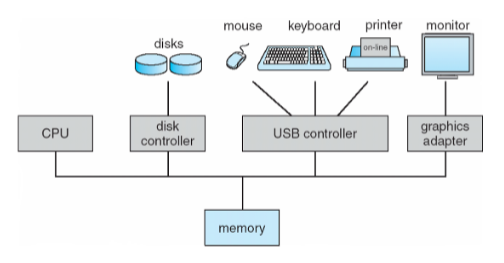
\includegraphics[scale=0.5]{fig1}
\end{center}
One or more CPUs or device controllers connect through a common bus, providing access to shared memory. CPUs and devices compete for memory cycles (i.e. to read and write memory addresses).

\end{document}
